\subsection{Background of QUIC}

\begin{comment}
\subsection{Dynamic adaptive streaming over HTTP(DASH)}
DASH provides a standard solution for the efficient and easy streaming of multimedia using existing available HTTP infrastructure (particularly servers and CDNs, but also proxies, caches, etc.). DASH specification provides a full set of HTTP adaptive bitrate streaming features for delivering multimedia over Internet.The features include the following:\footnote{\url{https://www.wowza.com/forums/content.php?508-How-to-do-MPEG-DASH-streaming} (\lastaccessedtoday)}
\begin{itemize}
	\item Frame-synchronized adaptive bitrate switching.
	\item Codec-agnostic.
	\item DRM-agnostic. It specifically supports the Common Encryption (CENC) system.
	\item Evolving support for closed-captions and subtitles.
	\item Support for multiple file container formats.
	\item Support for multiple manifest formats for VOD and live streaming.
	\item Fast-growing industry support.
\end{itemize}

A DASH server provides client players with a list of the available media chunk URLs in a \textit{Media Presentation Description (MPD)} manifest file.

\end{comment}
%Today, the web is the most widely used service over the Internet where HTTP is used to transfer the content of a web page from the web server to the web client which is typically a browser.
%It serves pages to a client using application layer protocol HTTP.
%HTTP1.1~\cite{RFC2616} uses a request-response method, and almost each request requires a new TCP connection from the client to the server and vice versa.
%However, the current websites may require as many as $100$ objects to be fetched to render a page properly. If every HTTP request requires a new TCP connection,
%Therefore, a significant amount of time needs to be spent only on  TCP connection establishment. Further, most of the today's secure web-servers uses the TCP+TLS protocol stack (as shown in \fig\ref{fig:quic-protocolstack}), where {\em Transport Layer Security} (TLS) is used to establish the end-to-end secure tunnel between the server and the client. TLS needs one additional round trip time (RTT) for the server-client handshaking for security parameter exchange.
To solve the problems of connection setup and \ac{TLS} handshaking delay for every \ac{HTTP} request-response flow, Google introduced a new protocol in 2012, called  \acsu{SPDY}~\cite{SPDYingupweb,Erman} that can multiplex more than one \ac{HTTP} requests/responses into one \ac{TCP} connection. Although \acsu{SPDY} reduces the connection establishment time, however, due to \ac{TCP}'s in-order packet delivery, all the \ac{HTTP} streams in a multiplexed \ac{TCP} connection get blocked with \ac{SPDY} even for a single packet drop event from any one of the \ac{HTTP} streams, which is known as \ac{HoL} blocking problem. To address \ac{HoL} blocking, Google has introduced another new experimental protocol called \ac{QUIC}~\cite{roskind2015quic,Cui2017,Megyesi2016} that uses \ac{UDP} based multiplexed streaming to provide low latency connections for web access. As shown in \fig\ref{fig:quic-protocolstack}, \ac{QUIC} uses \ac{UDP} as the underlying transport layer protocol to solve the \ac{HoL} blocking issue with \acsu{SPDY}, and therefore it has its own congestion control and flow control mechanisms~\cite{Cui2017,roskind2015quic}. The key benefits of \ac{QUIC} over \ac{TCP}+\ac{TLS} are as follows -- (a) reduction in connection establishment latency, (b) multiplexing of multiple application flows without head-of-line blocking, (c) improved congestion control over multiplexed application flows, (d) forward error correction for low latency communication, and (e) connection migration to support seamless mobility in the network.

\begin{figure}[!t]
	\centering
	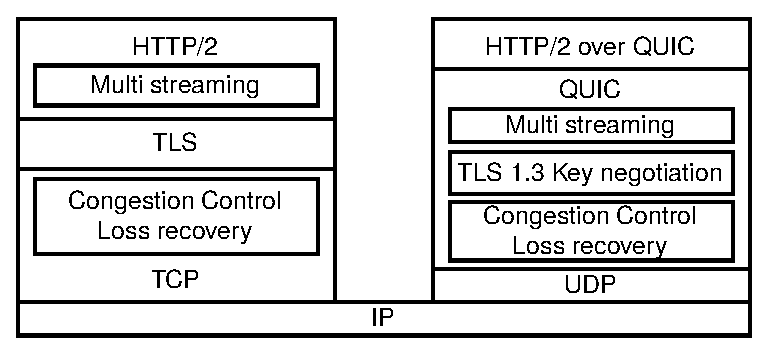
\includegraphics[width=0.7\linewidth]{img/quic-protocolstack}
	\caption{\acs{QUIC} Protocol Stack}
	\label{fig:quic-protocolstack}
\end{figure}

%\subsection{Quick UDP Internet Connections (QUIC):}

%It does not suffer from HoL blocking as it uses UDP as the transport protocol.
%As shown in \fig\ref{fig:quic-protocolstack}, unlike current TCP+TLS stack, QUIC does not require any separate TLS handshaking~\cite{Cui2017,roskind2015quic}. It can perform security handshaking during connection establishment only~\cite{Cui2017,Megyesi2016}. QUIC uses a congestion control algorithm similar to TCP, which are either TCP Reno, TCP New-Reno or TCP Cubic~\cite{Cui2017,roskind2015quic}.
%QUIC also uses a {\em forward error correction} (FEC) technique to reconstruct a lost packet in the network through redundant data transmission over multiple packets.
%This reconstruction is required to maintain QUIC philosophy of low latency connection. QUIC has been deployed in Google Chrome browser and Chromium browser.

Recent studies~\cite{Megyesi2016, Carlucci,Lychev2015,Biswal2016} on the performance of \ac{QUIC} have revealed that \ac{QUIC} can improve the web performance by reducing page load time even at poor network conditions.
%Next, we give a summary of the related works that have studied the performance of QUIC under various scenarios.
%Modern web run on top of TCP+TLS stack (\fig\ref{fig:quic-protocolstack}). This two stack have their own connection establishment time. As web need a lot of short-lived HTTP connections, this establishment time is huge part of their overall life time. To mitigate these problems, Google has developed QUIC.
%
%QUIC solves a number of transport-layer and application-layer problems including the one we mentioned earlier, experienced by modern web applications, while requiring little or no change from application writers. QUIC is very similar to TCP+TLS+HTTP2, but implemented on top of UDP. Having QUIC as a self-contained protocol allows innovations which are not possible with existing protocols as they are hampered by legacy clients and middleboxes.\footnote{\url{https://www.chromium.org/quic} (\lastaccessedtoday)}\\\\
%\noindent
%Key advantages of QUIC over TCP+TLS+HTTP2 include:
%\begin{itemize}
%	\item Connection establishment latency
%	\item Improved congestion control
%	\item Multiplexing without head-of-line blocking
%	\item Forward error correction
%	\item Connection migration
%\end{itemize}
%\begin{figure}
%    \centering
%    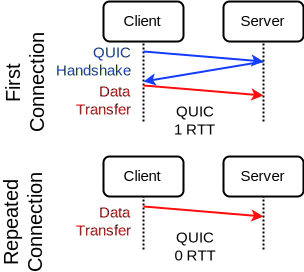
\includegraphics[width=0.7\linewidth]{img/quicrtt}
%    \caption{}
%    \label{fig:quicrtt}
%\end{figure}
%\subsection{Related Works}
%Most of the previous works in QUIC compare its performance with HTTP1.1 and SPDY~\cite{qian2015toward,Megyesi2016, Carlucci,Lychev2015,Biswal2016,bakri2015http}.
In \cite{Cui2017}, Cui \textit{et. al.} have shown that \ac{QUIC} has the potential to change the web and make it faster and more secure.
%as they have shown the improved performance of QUIC compared to various other end-to-end protocols.
Megyesi \textit{et al.}~\cite{Megyesi2016} have compared \ac{QUIC} with \acsu{SPDY} and \ac{HTTP} and found that \ac{QUIC} outperforms those protocols for web access under low network bandwidth availability. However, they have also noted that \ac{QUIC} does not work well with the large objects, such as large file transfer. In \cite{Biswal2016}, Biswal \textit{et al.} have found that \ac{QUIC} can load web pages much faster than HTTP2.0. They have also shown that \ac{QUIC}'s performance increases with increasing size of object and number of objects on a page, which is little contrary to the observation given by \cite{Megyesi2016}. Lychev \textit{et al.}~\cite{Lychev2015} have analyzed security aspects of QUIC and have presented the first security model for \ac{QUIC}. They have found that simple bit-flipping and replay attack can prevent \ac{QUIC} from achieving its goal of low latency. They have also claimed that this weakness is there because of the goal of low-latency. In~\cite{bakri2015http}, the authors have developed a service for multi-user virtual world by exploring the low latency features of HTTP2.0 and \ac{QUIC}.

In summary, most of these works claim that \ac{QUIC} has the proficiency to improve the performance of web access.
% As most of today's streaming services work on top of HTTP, like YouTube, NetFlix and so on,
Therefore, it would be interesting to see how web based video streaming services perform when the underlying \ac{TCP}+\ac{TLS} stack is replaced by \ac{QUIC}. However, to the best of our knowledge, no recent work has looked into web based adaptive streaming performance over \ac{QUIC}.
%In this paper, we investigate this performance issues by looking into a widely used streaming service, YouTube.

%Most of the work done on QUIC was how QUIC performs with respect to TCP and SPDY in terms of page load time. In \cite{citation-1-name-here} they studied about the performance of QUIC, SPDY and HTTP particularly about how they affect page load time. They found that none of these protocols is clearly better than the other two and the actual network conditions determine which protocol performs the best. Similarly in \cite{citation-6-name-here} they found out that QUIC reduces the overall page retrieval time with respect to HTTP in case of a channel without induced random losses and outperforms SPDY in the case of a lossy channel. The FEC module, when enabled, worsens the performance of QUIC.
%Almost all the research was concentrated on how QUIC performs in terms of page load time, the number of RTT's required and how it deals when there is packet loss so basically they were concerned about object transfers or static elements transfer and there were no major publications on how QUIC performs if it used for video streaming services like YouTube.

